\begin{figure}[H]
    \centering
    \setkeys{Gin}{width=\linewidth}
    \centering
        \begin{tabularx}{\textwidth}{YY}
            \textbf{Original fluorescence} &
            \textbf{Segmentation} \\
            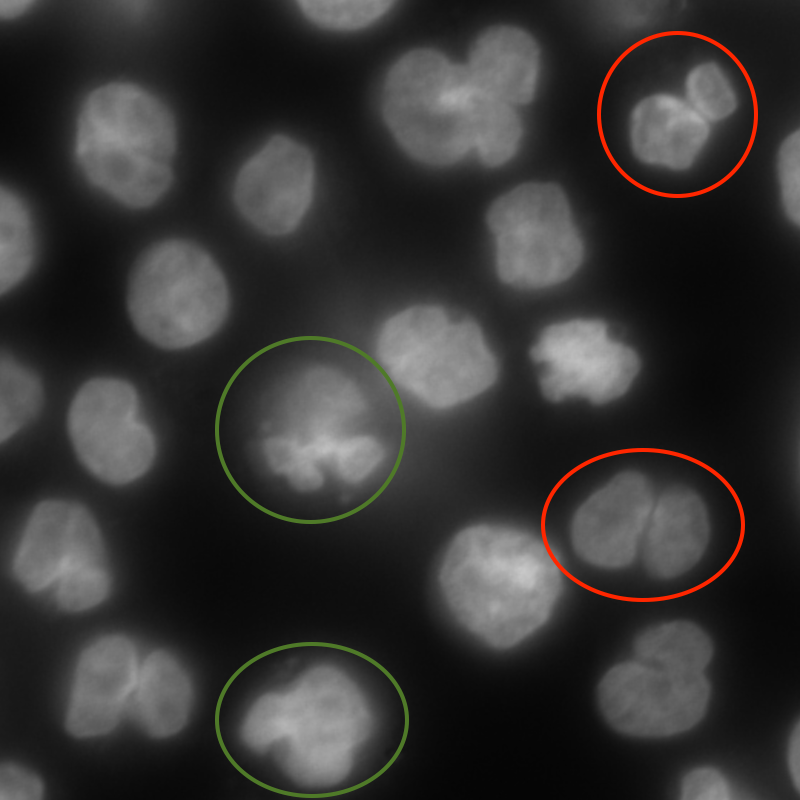
\includegraphics{bilder/close-located-cells/original.png} & 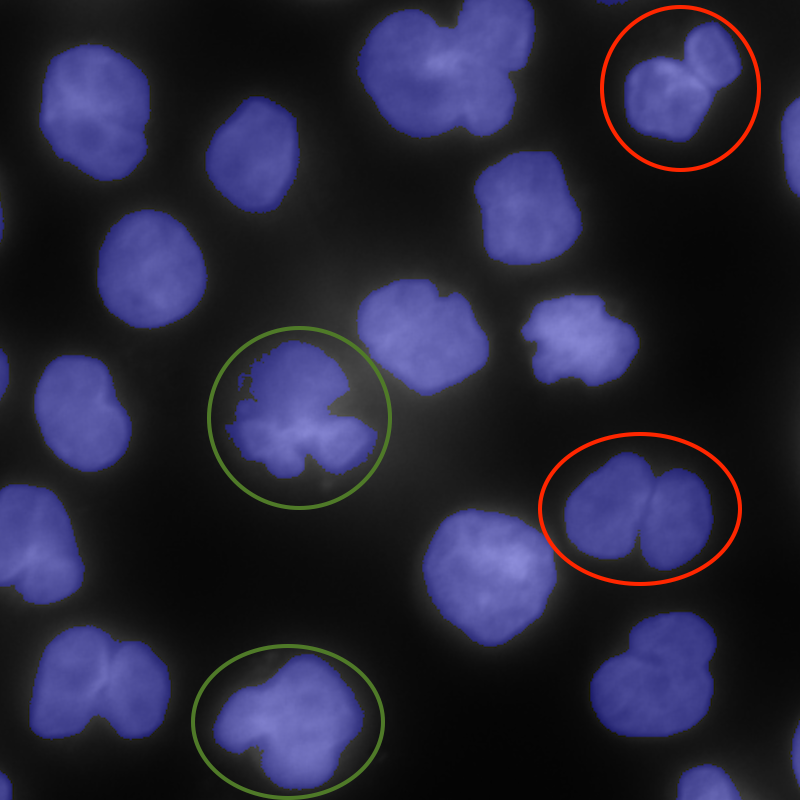
\includegraphics{bilder/close-located-cells/segmented.png}
        \end{tabularx}
    \caption{Closely located cells}
    \label{fig:closely-located-cells}
\end{figure}

Overall algorithm
\begin{figure}[H]
    \centering
    \setkeys{Gin}{width=\linewidth}
    \centering
        \begin{tabularx}{\textwidth}{YYYY}
            \textbf{Normalized input} &
            \textbf{Local threshold} &
            \textbf{Filled holes} &
            \textbf{Filtered regions} \\
            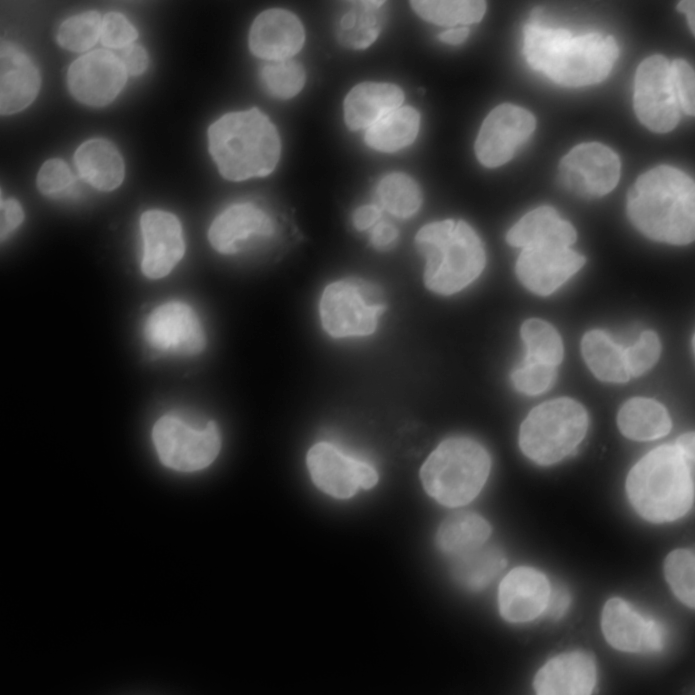
\includegraphics{bilder/segmentation/nuclei-mask/normalized.png} & 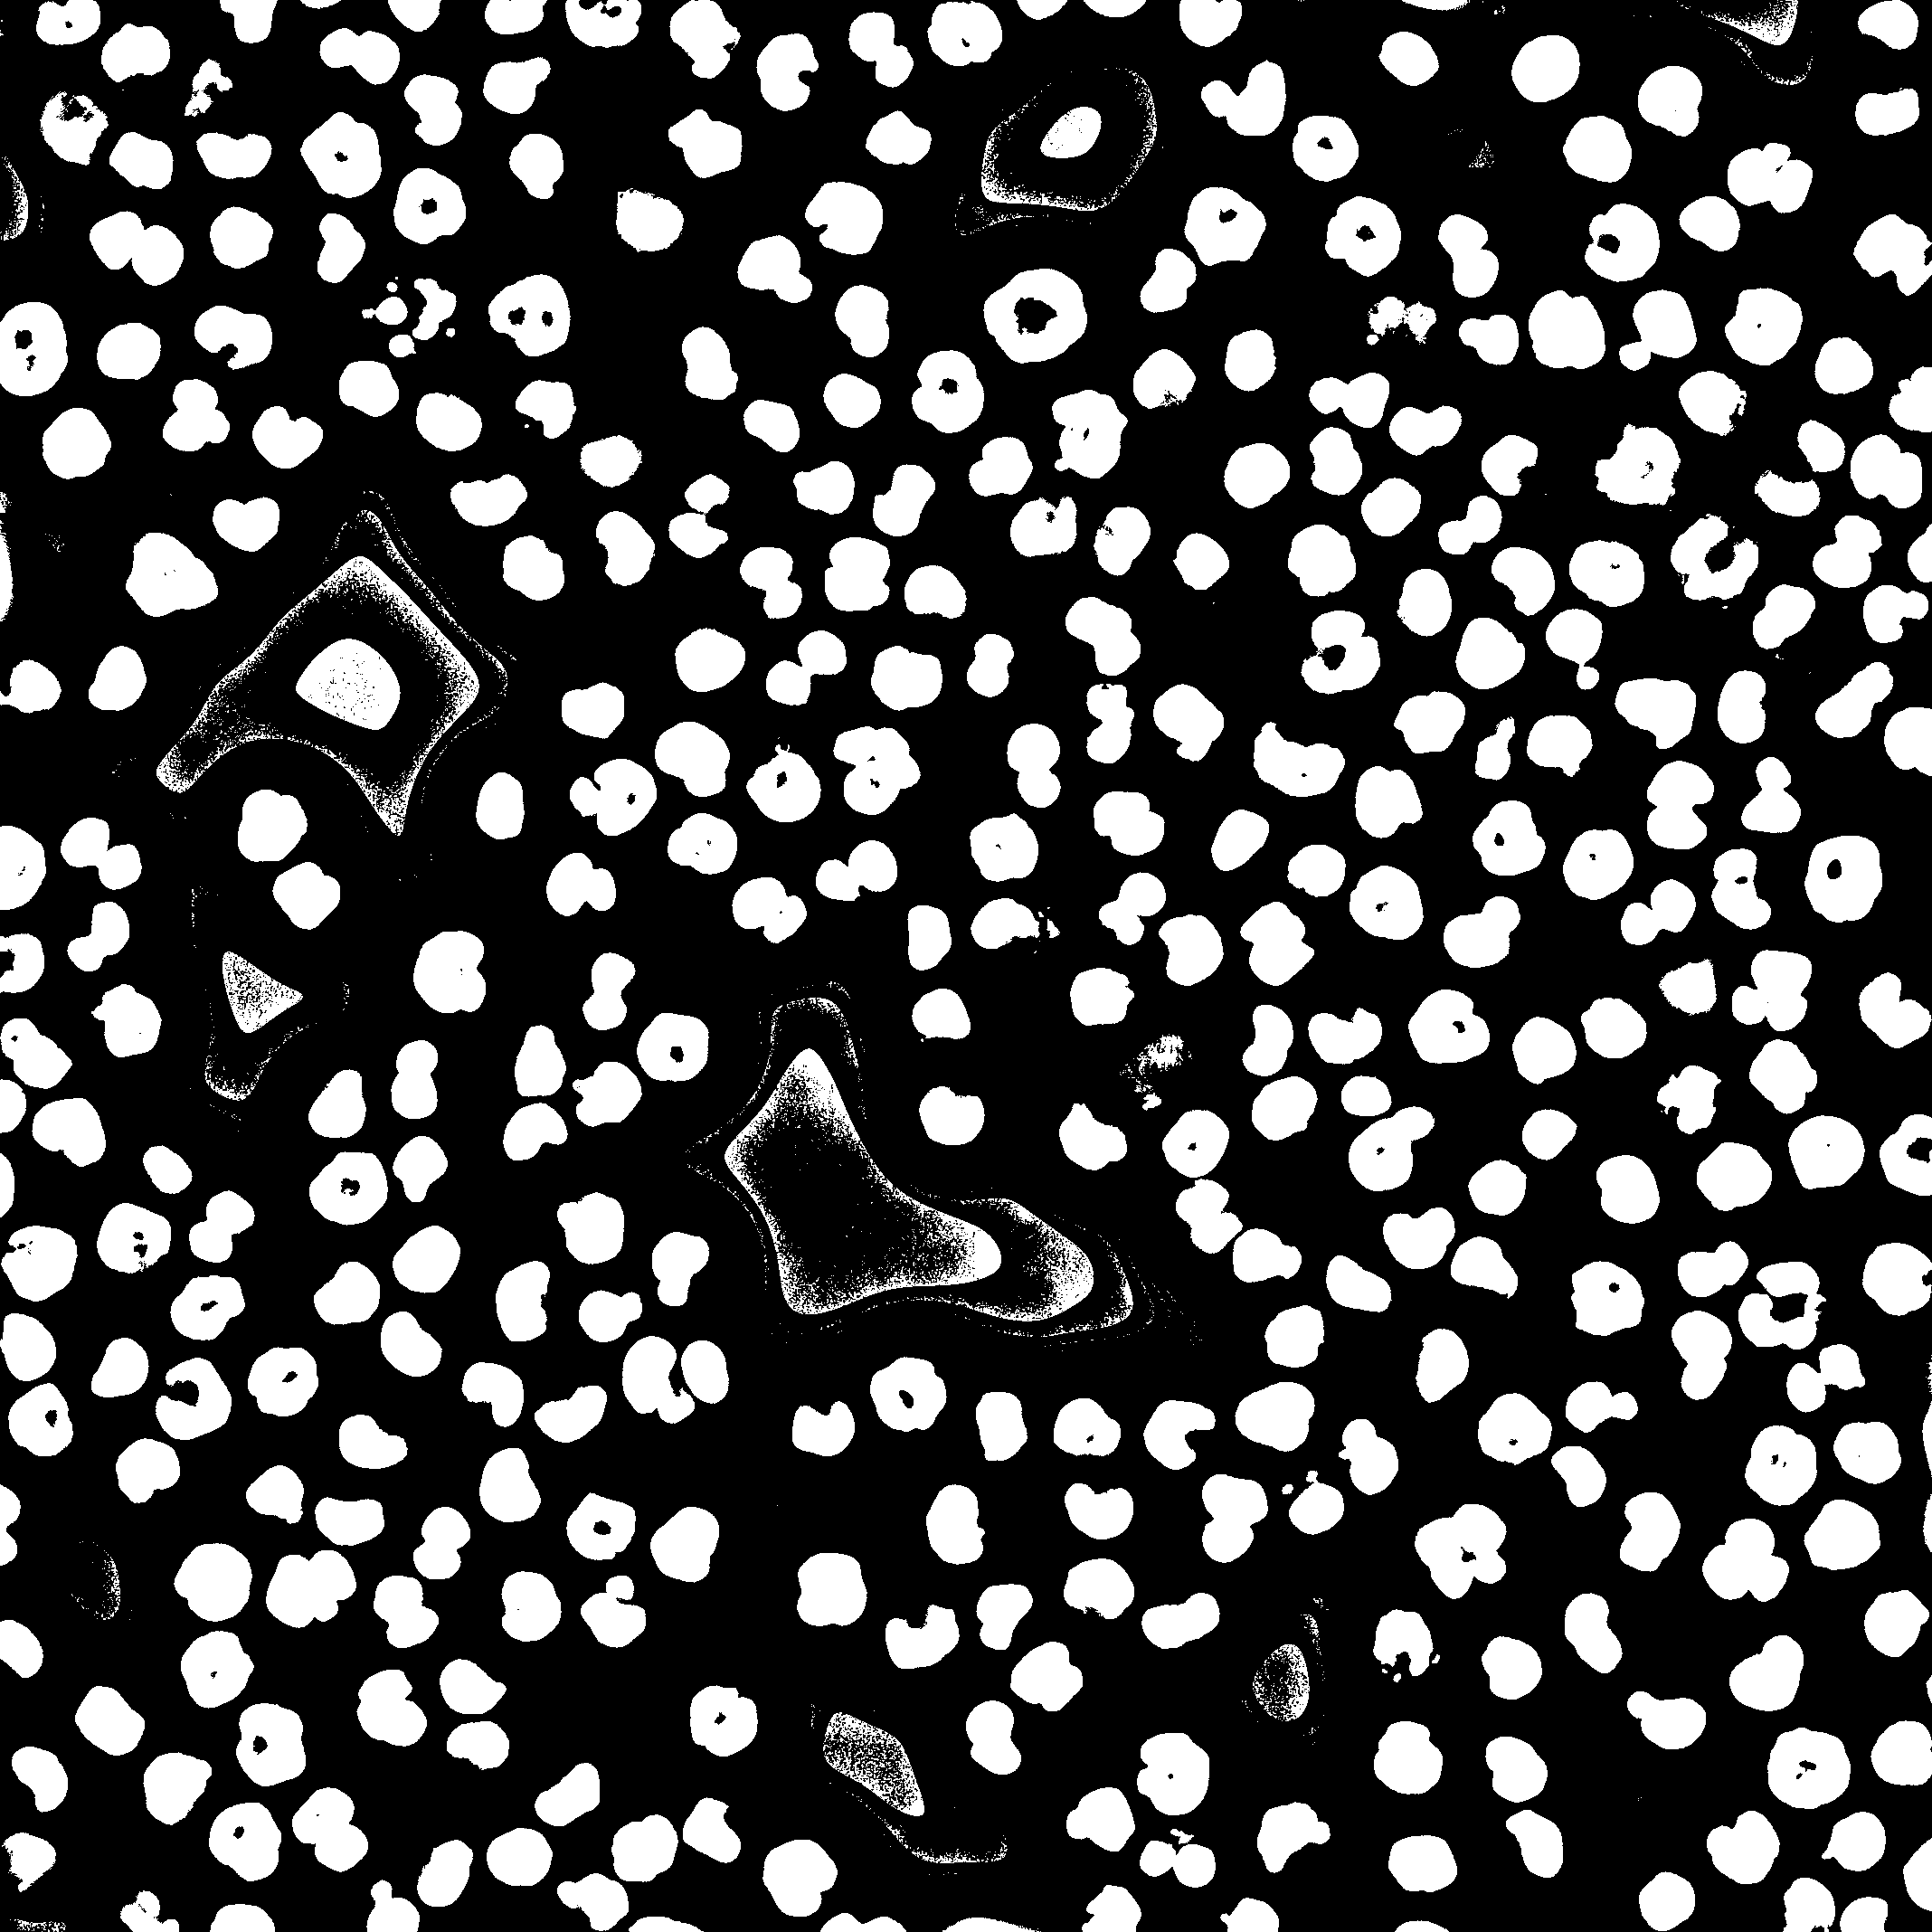
\includegraphics{bilder/segmentation/nuclei-mask/binary_local.png} &
            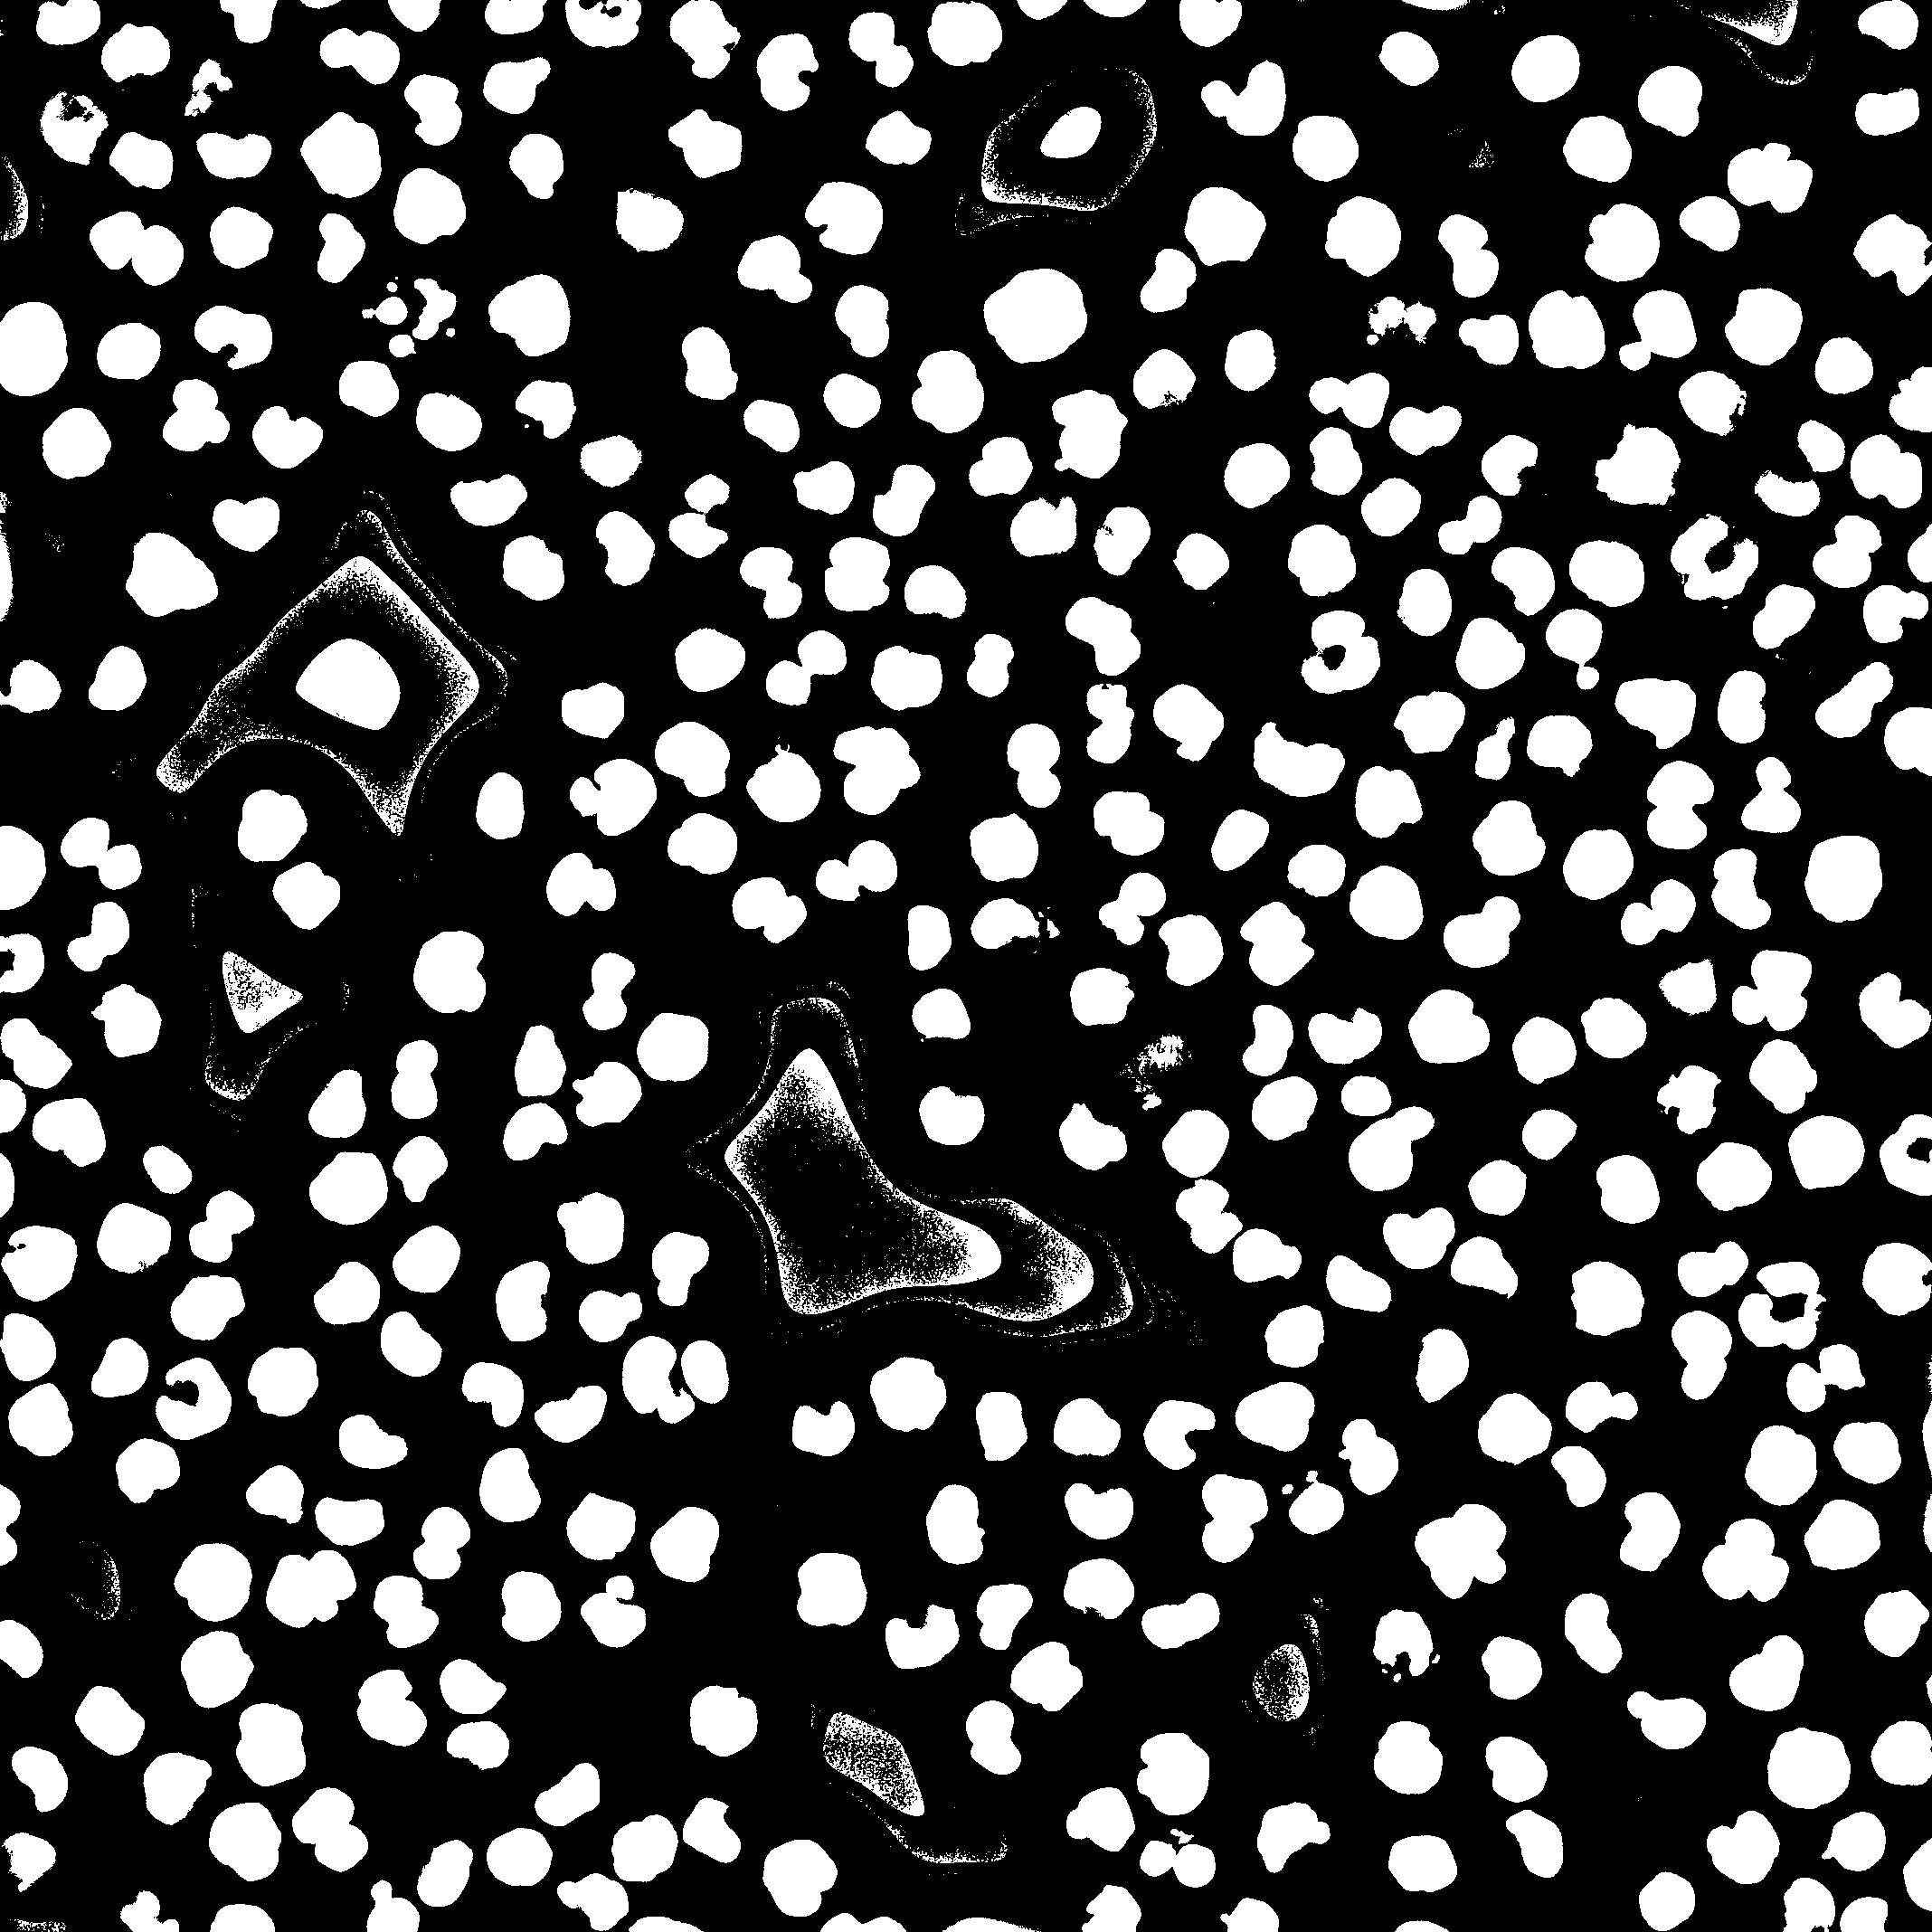
\includegraphics{bilder/segmentation/nuclei-mask/filled_holes.png} & 
            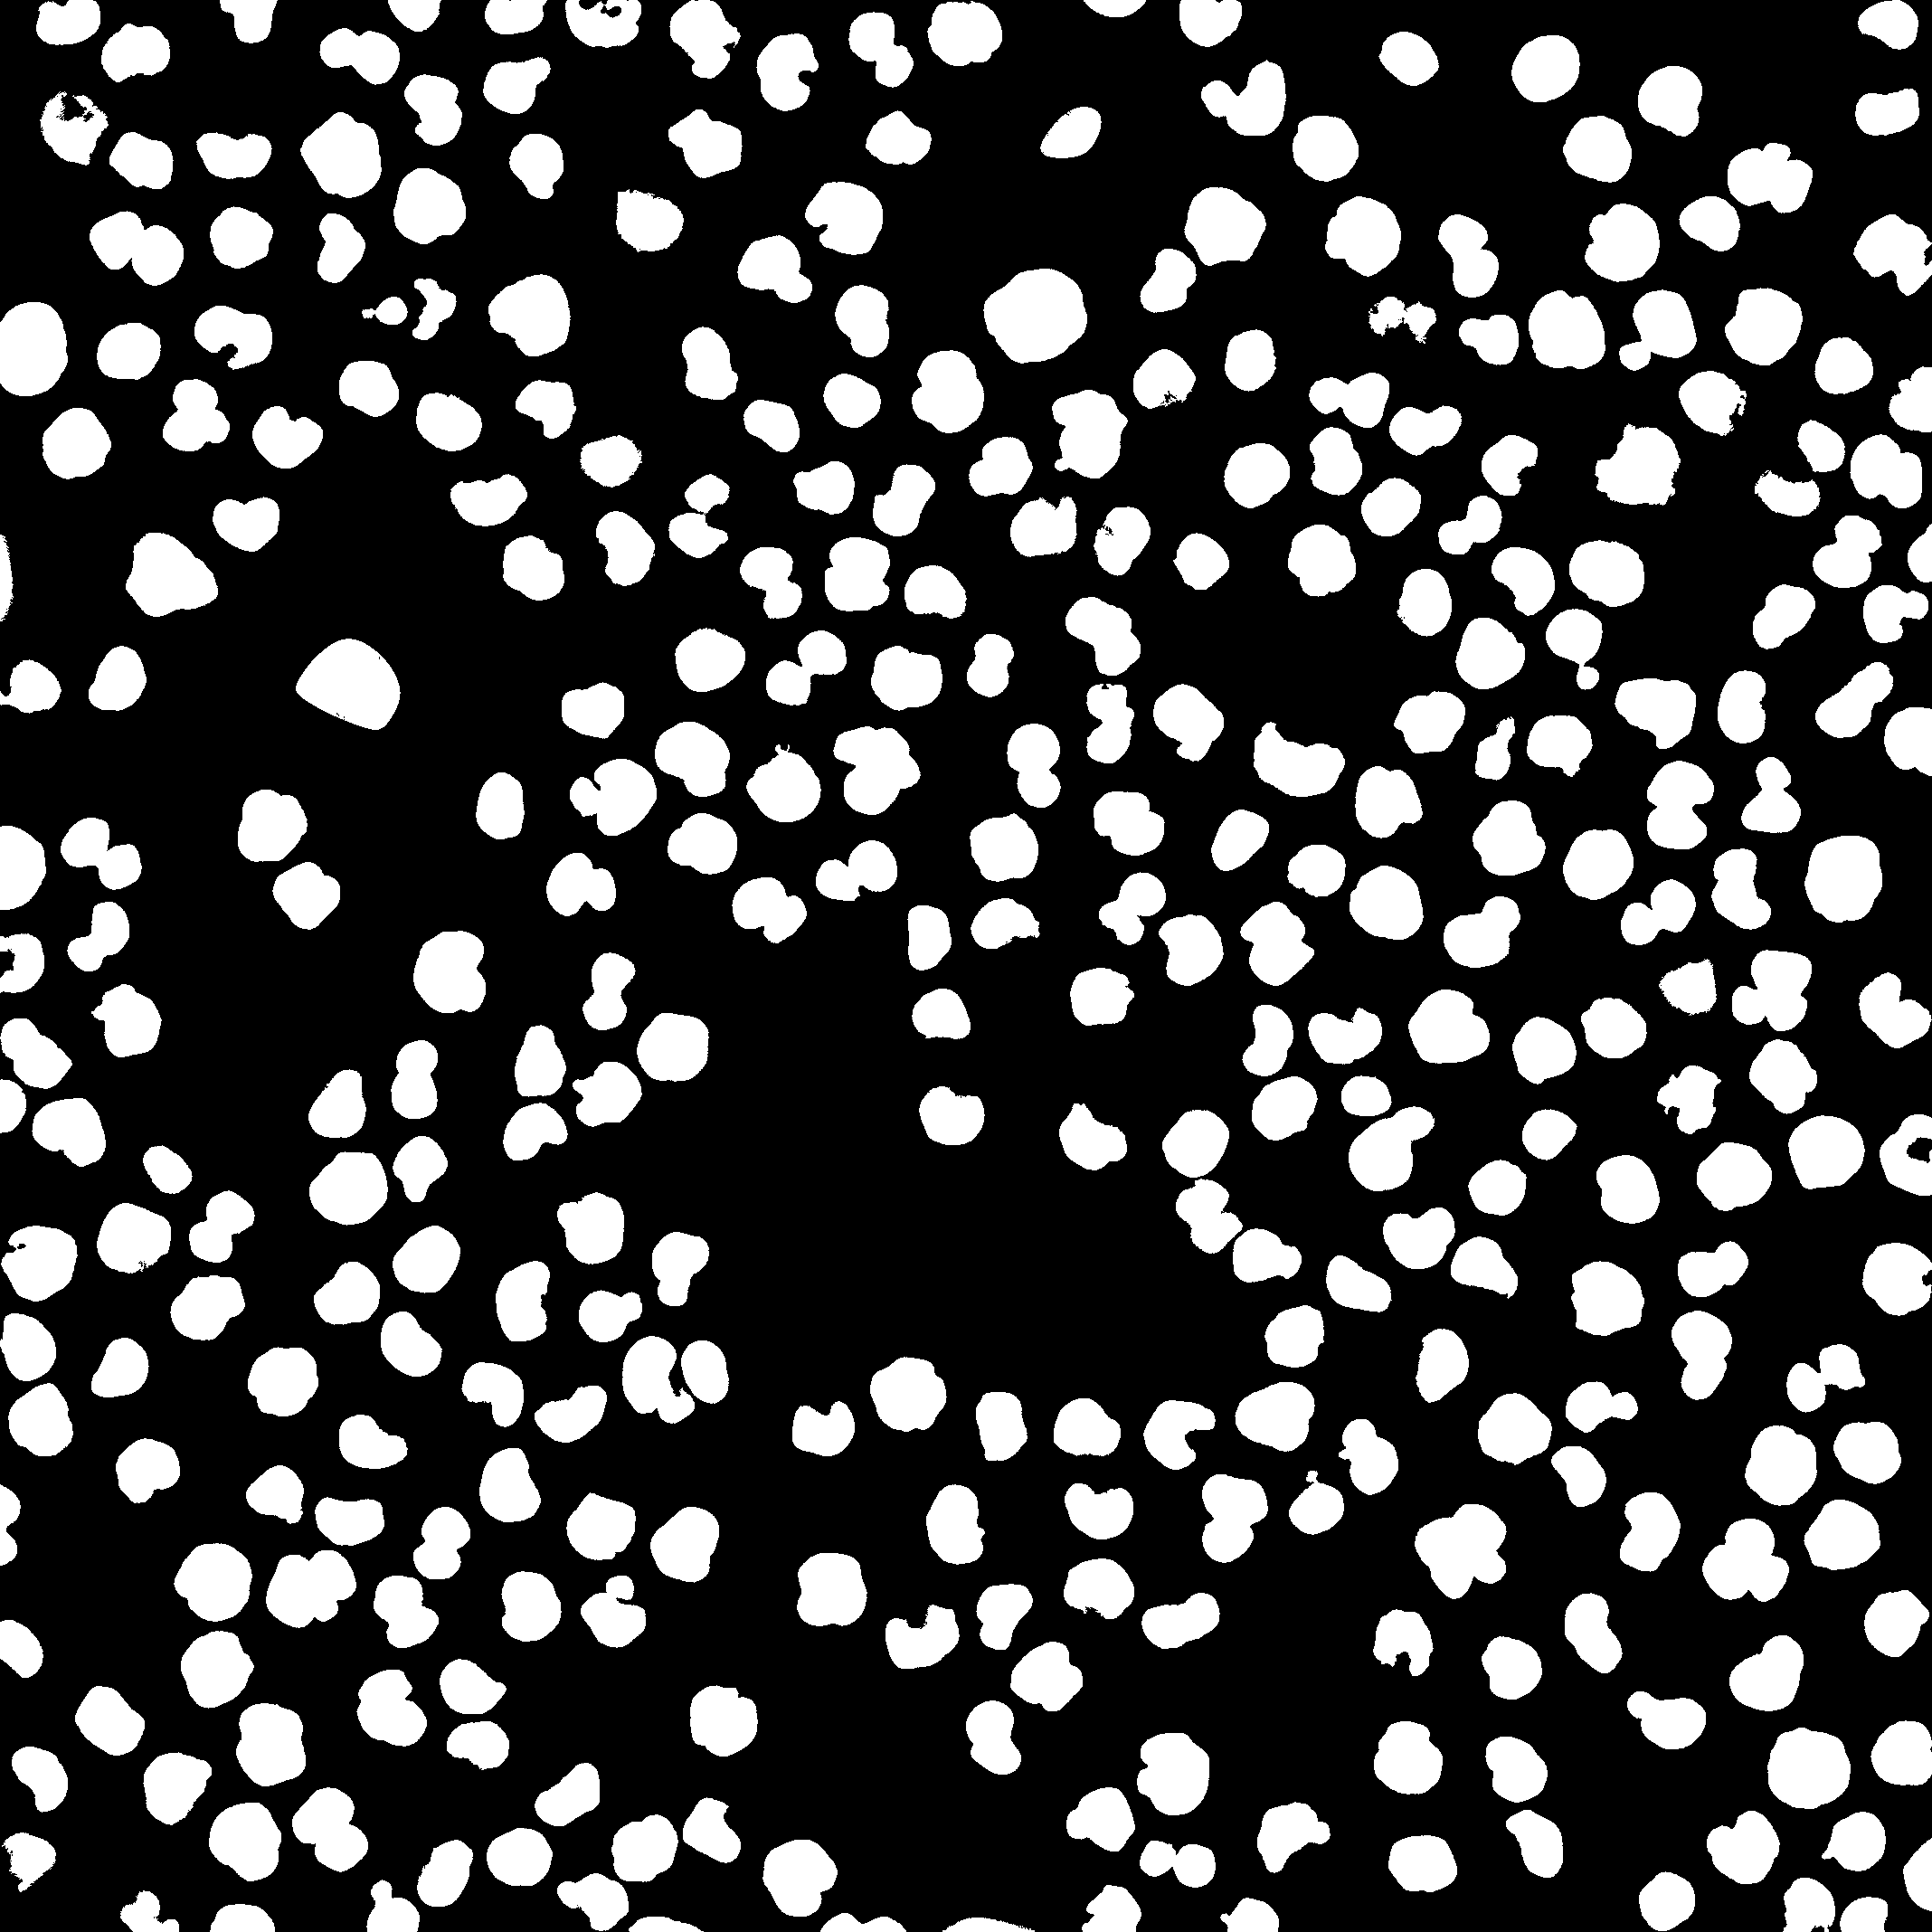
\includegraphics{bilder/segmentation/nuclei-mask/mask.png}
        \end{tabularx}
    \caption{Fluorescence segmentation}
    \label{fig:segmentation-nuclei-steps}
\end{figure}